\documentclass{article}
\usepackage[utf8]{inputenc}
\usepackage{graphicx}
\usepackage{appendix}
\usepackage{braket}
\usepackage{amsmath}
\usepackage{biblatex}
\addbibresource{references.bib}

\title{PHYS 593 Report}
\author{Yanjun Jin}
\date{04/27/2021}

\begin{document}

\maketitle

\section{Introduction}
As a new and rapidly developing field of study, quantum computing possesses the potential to significantly decrease the time it takes to solve a variety of problems. With its idea first being proposed in 1980s, there has been a lot of algorithms specifically designed for quantum computation. In the first section, we will discuss one such algorithm that brings out an interesting property of quantum computing. Additionally, due to the lack of physical quantum computers, many quantum computing algorithms and codes are being run on quantum computing simulators. In the next part of the report, we will be analysing the performance and the constraint of Qiskit (See Appendix A), a quantum computing framework for Python, developed by IBM. Noise and error correction in quantum circuits will be explored in the next section, where custom noise modules were used to test the effectiveness against a 9-qubit surface code. In the last section, we will briefly talk about a minimal quantum computing simulator we developed for Haskell.

\section{Symmetry of CX and CZ gates}

When researching the Bernstein-Vazirani algorithm - an algorithm that involves an oracle containing a hidden bit string and having to figure out what the bit string is without peeking into the oracle, an interesting X-Z symmetry was discovered. The oracle itself contains a bit string of set length, and it takes an input of the same length and output the original input and a bit 0 or 1 representing the sum of bit string and operation of the input and the hidden string modulo 2. 

The classical computer could find the number in tries of the number of digits. It can accomplish this by consecutively inputting strings that are inputting bit strings with all positions but one being 0. If the return value is 0, that bit is 0, if the return value is 1, that value is 1. Doing so repeatedly for all digits will allow the hidden bit string to be constructed bit-by-bit. In contrast, quantum computer can find the number in one single try. a quantum computer, an oracle could be constructed using controlled not gates on the output qubit using the input qubits as controls. To figure out the hidden number, all one needs to do is to apply Hadamard gates on all qubits (including output qubit) before and after passing into the oracle. The output bit string will be the hidden bit string.

According to Ref.\cite{paulsearleBernsteinVaziraniAlgorithmProgramming2019}, the reason the algorithm works is because the "Hadamard gate magic" that passes all inputs simultaneously. However, this explanation is not particularly satisfactory. After some experimentation a different explanation was found, being that a controlled X gate is in fact, a reversed controlled Z gate, and acts on, instead of the basis of $\ket{0}$ and $\ket{1}$, the basis of $\ket{+}$ and $\ket{-}$, and only performs Z operation of the target qubit when the controlled qubit is in $\ket{-}$ state. The permits the original controlled X gates in the oracle to function as a controlled Z in reverse, phase shifting the bits corresponding to $\ket{1}$ bits of the hidden bit string. Therefore, as long as we apply Hadamard gate on all of the input qubits, and and controlled not gate on the syndrome measurement qubit, we will essentially re-purpose the original oracle to act as a function that outputs its hidden bit string on the basis of $\ket{+}$ and $\ket{-}$. 

This symmetry is also consistent with the original functionality of a controlled not gate. This includes the following operations (the first qubit will be the control qubit):\newline
\begin{equation}
    \ket{00} \xrightarrow{CNOT} \ket{00}
\end{equation}
\begin{equation}
    \ket{01} \xrightarrow{CNOT} \ket{01}
\end{equation}
\begin{equation}
    \ket{10} \xrightarrow{CNOT} \ket{11}
\end{equation}
\begin{equation}
    \ket{11} \xrightarrow{CNOT} \ket{10}
\end{equation}

Consider the X-Z symmetry, also using first qubit as control, we must also obtain:
\begin{equation}
    \ket{00} \xrightarrow{CZ} \ket{00}
\end{equation}
\begin{equation}
    \ket{01} \xrightarrow{CZ} \ket{11}
\end{equation}
\begin{equation}
    \ket{10} \xrightarrow{CZ} \ket{10}
\end{equation}
\begin{equation}
    \ket{11} \xrightarrow{CZ} \ket{01}
\end{equation}

Using the equations: 
\begin{equation}
    \ket{0} = \frac{1}{\sqrt{2}} \ket{+} + \frac{1}{\sqrt{2}} \ket{-}
\end{equation}
\begin{equation}
    \ket{1} = \frac{1}{\sqrt{2}} \ket{+} - \frac{1}{\sqrt{2}} \ket{-}
\end{equation}

The above relationships could be easily proven to be true using simple algebra.

This symmetry in controlled X and Z operations warrants further investigation and could be an interesting topic in building quantum algorithms.
\newpage
\section{Run-time}

Another topic that was touched on was the run-time of quantum circuits that are simulated using classical computers. This section is dedicated to the evaluation to the performance and run time of the quantum assembly simulator, or qasm, which is a component of IBM Qiskit under package Aer (See Appendix A). To analyze the run-time of simulating non-Clifford gate on qubits, a quantum circuit that involves T gates and Toffoli gates was built, which scales linearly with the number of qubits it has. The time was recorded using $timeit$ package. For every 3 qubits, T gates were applied to the first and the third qubits. Then a Toffoli gate was applied onto the first qubit, using the second and the third qubits as control. If there are less than 3 qubits left in the end, the Toffoli gate will not be applied. After the Toffoli gate, a T gate is applied to the first qubit. In the end, a CNOT gate is applied using the third qubit as control onto the first qubit of the next triplet. This chunk can be repeated for a set of repetitions for one's choosing. At the end of the circuit, T and S gates are applied to all qubits. All qubits are measured and the results are stored in classical registers. Figure 1 illustrates a 6 qubit situation:

\begin{figure}[h]
    \centering
    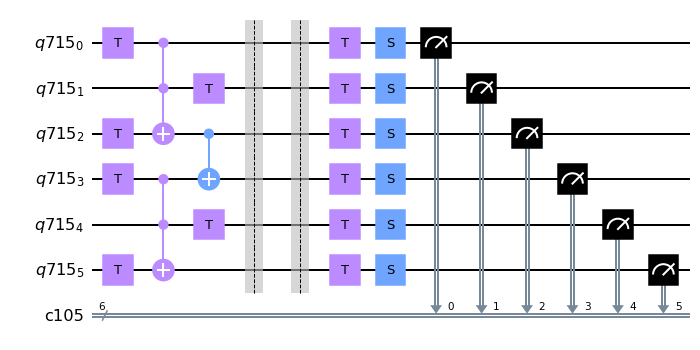
\includegraphics[width = 0.8\linewidth]{runtime/6qubit.png}
    \caption{6 qubit code}
    \label{fig:my_label}
\end{figure}

The test run involves repeatedly building circuits that involve 1 to 27 qubits, each running 1024 repetitions and has 1 repetition of the chunk. This yields a curve that looks exponential as demonstrated in Fig 2.

\begin{figure}[p]
    \centering
    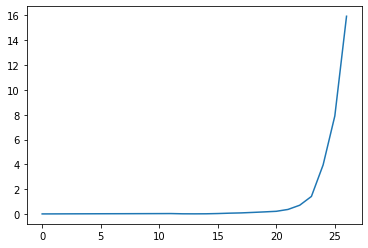
\includegraphics[width = 0.8\linewidth]{runtime/1-27 1.png}
    \caption{Run-time for 1 to 27 qubits. The x-axis denotes the number of qubits in the circuit; the y-axis denotes run-time in seconds.}
    \label{fig:my_label}
\end{figure}

This is evident when we map $\log$ to the time variable in Figure 3.

\begin{figure}[p]
    \centering
    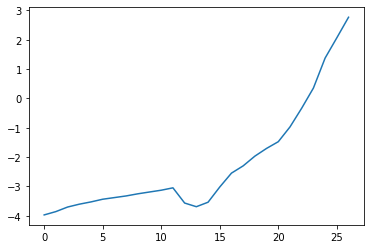
\includegraphics[width = 0.8\linewidth]{runtime/1-27 1log.png}
    \caption{Applying natural log to run-time.  The x-axis denotes the number of qubits in the circuit; the y-axis denotes logarithmic run-time in seconds.}
    \label{fig:my_label}
\end{figure}

The patterns look the same no matter how many logarithms are applied. The action of adding e each time could potentially constitute to some deviation, but if any term is growing slower than exponential, the convex graph should eventually become concave. It seems to imply that, for this specific simulation method and circuit, the computation time increases more than just exponentially.

It seems anything larger than 29 qubits results in the qasm simulator not responding and crashing during calculation. This is caused by the memory limitation. Increasing the maximum buffer size of Jupyter Notebook only allows a simulation of 32 qubits, and a maximum of 32GB of RAM is used despite 90GB of ram it is allowed to occupy.

Another simulation was built to investigate how more repetitions constitutes to the run-time. The test was run on 9 qubits from 1 to 100 chunk repetitions. Each chunk consists of the block of T gates and Toffoli gates mentioned previously. There seems to be anomaly spikes during the run as shown in the plot below. We could say with relative confidence that at 0-20 repetition, the run-time scales linearly with $\Theta(n)$. After the first spike the minimum run-time seems to increase linearly, but at a slower pace, as illustrated in Figure 6. The cause of the spikes could be due to caching/RW operations of the qasm algorithm, and that is what caused the run-time to spike and subsequent runs to take less time. However, the spikes are more frequent the more repetitions are added. This is evident on the run with 1-250 repetitions (Figure 7), where the highs and lows of the spikes seems to be linearly scaling with the number of repetitions.

\begin{figure}[p]
    \centering
    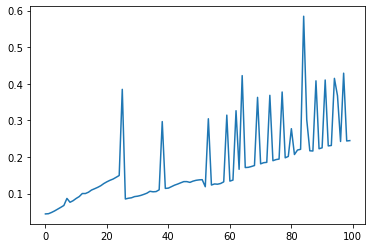
\includegraphics[width = 0.7\linewidth]{runtime/9 1-100.png}
    \caption{Run-time of 1 to 100 Chunks. The x-axis denotes the number of chunk repetitions; the y-axis denotes run-time in seconds.}
    \label{fig:my_label}
\end{figure}

\begin{figure}[p]
    \centering
    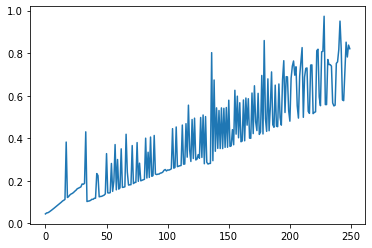
\includegraphics[width = 0.7\linewidth]{runtime/9 1-250.png}
    \caption{Run-time of 1 to 250 Chunks. The x-axis denotes the number of chunk repetitions; the y-axis denotes run-time in seconds.}
    \label{fig:my_label}
\end{figure}
\newpage
\section{Noise Generation}

There are two ways to generate noise in Qiskit. One is to fetch existing noise parameter from the IBM physical machines. This is done by obtaining the device properties of the backend. This noise model includes a set of basis gates, instructions with noise, qubits with noise, and specific qubit errors. How it work seems to be converting the QuantumError into a set of gates and instructions that each has a probability to apply whenever a gate is applied. One could obtain the specific probability and error types by printing after converting the noise model to dictionary using the $to\_dict()$ function. There does not seem to be any other function to obtain the noise type and probability native to Qiskit, so converting to dictionary is a workaround to obtain the fundamental properties of the noise model. 

One could also build custom noise models by using built in functions to apply certain errors (Pauli error, for example) on one or more gate using\newline
$add\_all\_qubit\_quantum\_error()$ method by specifying the probability that each error may occur during the application of each gate. The error could also be applied to classical operations including reset and measure. However, there is no native method to simulate the decay of quantum states overtime. In this case, a custom model for id gate could be built so that simulation of time-dependent qubit specific error is possible. This is illustrated by building a circuit composing a series of id gates as shown in Figure 8.

\begin{figure}[p]
    \centering
    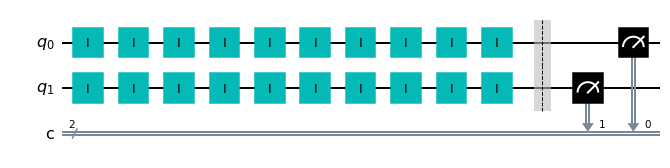
\includegraphics[width = 0.8\linewidth]{noise/id.png}
    \caption{Circuit to simulate Pauli noise over time. $I$ gates here denotes id gates, which is set to be susceptible to Pauli noise.}
    \label{fig:my_label}
\end{figure}

The end result has noise on both qubits, resulting in measurements other than $\ket{00}$ states.

\begin{figure}[p]
    \centering
    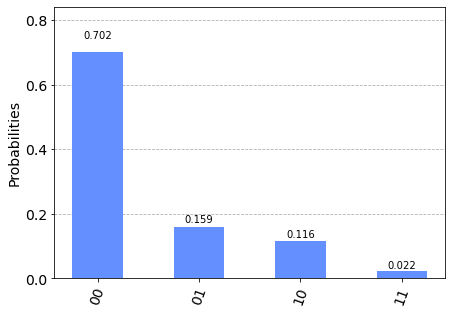
\includegraphics[width = 0.8\linewidth]{noise/noise.png}
    \caption{Result of the noise simulation circuit. The x-axis denotes the resulting states, the y-axis denotes number of occurrences.}
    \label{fig:my_label}
\end{figure}
\newpage
\section{Surface Code}

A surface code constructed as a grid with nine vertices will be built for the purpose of investigating the concrete implementation of quantum error correction. For this 9-qubit surface code, there is a qubit on each vertex that encodes a bit. The center of each grid has a syndrome measurement, interlacing X and Z, the top-left grid is occupied by a Z-syndrome measurement. For each side, an X or Z syndrome measurement is also applied to the first two qubits, interlacing with the grid syndrome measurements, so that no two same syndrome measurements neighbor each other. This will be similar to the surface code described in Ref.\cite{bravyiCorrectingCoherentErrors2018}, but will be rotated 90 degrees. With the top left plaquette taking X instead of Z syndrome measurement, shown in Fig. 8.

\begin{figure}[h]
    \centering
    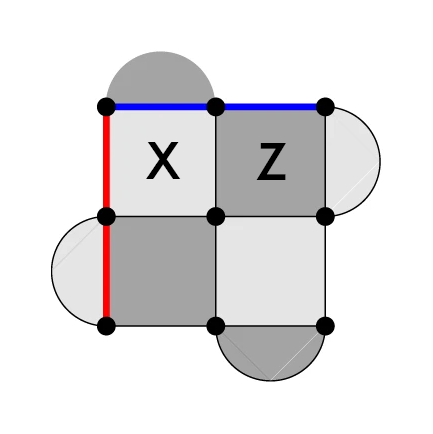
\includegraphics[width = 0.7\linewidth]{surface/9-qubit.png}
    \caption{The 9-qubit surface code  we are constructing. The plaquettes of the same shade contains the same syndrome measurements. The blue line is the $X_{Logical}$ operation, while the red line is the $Z_{Logical}$ operation.}
    \label{fig:my_label}
\end{figure}

The first difficult problem of building and running said circuit was to find the eigenvectors. There are overall 9 data qubits and 8 syndrome measurement. Each ancilla bit (X or Z in the figure) has a stabilizer operator. These take form as tensor products of the simple gate applications on each qubit. When a syndrome measurement is performed, since the result can either be 1 or 0, it projects the statevector of the entire circuit onto either the +1 or -1 eigenspace of the stabilizer tensor. In this instance, we will be using matrices to represent these tensors for its ease of computation.

Initially, the data qubits will have, in total, $2^9$ states permissible. Each of the syndrome measurement will subdivide the vector space into two sub-spaces of eigenspace +1 and -1. Therefore, it is possible for two eigenvector to be found on the eigenspace of +1 of the syndrome. This provides two degrees of freedom of the circuit, which is essential to simulating logical $\ket{0}$ and $\ket{1}$ on the circuit scale. (Ref.\cite{zatloukalStabilizerCircuits})

The set of stabilizers of our 9-qubit surface code be:
\begin{equation}
    Z_0 \otimes Z_1 \otimes I \otimes I \otimes I \otimes I \otimes I \otimes I \otimes I
\end{equation}
\begin{equation}
    I \otimes Z_1 \otimes Z_2 \otimes I \otimes Z_4 \otimes Z_5 \otimes I \otimes I \otimes I
\end{equation}
\begin{equation}
    I \otimes I \otimes I \otimes Z_3 \otimes Z_4 \otimes I \otimes Z_6 \otimes Z_7 \otimes I
\end{equation}
\begin{equation}
    I \otimes I \otimes I \otimes I \otimes I \otimes I \otimes I \otimes Z_7 \otimes Z_8
\end{equation}
\begin{equation}
    X_0 \otimes X_1 \otimes I \otimes X_3 \otimes X_4 \otimes I \otimes I \otimes I \otimes I
\end{equation}
\begin{equation}
    I \otimes I \otimes X_2 \otimes I \otimes I \otimes X_5 \otimes I \otimes I \otimes I
\end{equation}
\begin{equation}
    I \otimes I \otimes I \otimes X_3 \otimes I \otimes I \otimes X_6 \otimes I \otimes I
\end{equation}
\begin{equation}
    I \otimes I \otimes I \otimes I \otimes X_4 \otimes X_5 \otimes I \otimes X_7 \otimes X_8
\end{equation}

Because all of these operators commute, they will have mutual eigenvectors. However, the eigenvalues might not be the same. Now the second problem of creating the entangled states is encountered.

The amount of calculation makes calculation by hand infeasible, so several programs were considered to aid the calculation. The original program used to perform the calculation was Wolfram Mathematica. However, we suspect that Wolfram Mathematica may not be able to handle some $2^{9^2}$ data efficiently, and it was relatively restricted in Wolfram Mathematica to manipulate data structures. In the end, python and numpy package is used to calculate the mutual eigenvectors of the syndrome.

The Kronecker product of each of the syndromes are calculated and stored in the corresponding arrays. The problem arises when attempting to extract the mutual eigenvectors of all syndrome measurements. The problem was that the native function for extracting elements, intersect1d(), flattens the entire array before making comparisons, so the result is only element-wise. It would also turn out that the function in numpy for eigenvectors do not return a list of eigenvectors, but instead returns an matrix with each column being an eigenvector. One major hurdle was that the basis of eigenspace is arbitrary, so there might not be a one-to-one match of the eigenvectors of different syndromes. We have to find the overlapping of the eigenspace spanned under identical eigenvalues.

A custom code was written to extract identical items within two arrays. However, it would turn out that there are no mutual eigenvectors between all the X syndrome measurements. Since we are looking for eigenvalues that are equal to 1, the array of eigenvalues of the X syndrome measurements represent the 1-eigenspace, which means any linear combinations of the eigenstates are also eigenstates of the syndrome measurements. Therefore, since the eigenstates we calculated is using an arbitrary set of basis eigenstates, we might not find the exact set of eigenstates that are identical matches to each other despite the fact that the subspace they span have overlap.

Understanding this, what we are currently trying to accomplish is to find a way to calculate the intersection between the space spanned by two sets of vectors. This implies that a certain linear combination of the first set of vector is equal to the second set of vector. So we can simply append the second matrix to the first, and calculate its null-space using singular-value decomposition. Calculating the null-space essentially answers the question of "What linear combination of the first set eigenbasis and the second set of eigenbasis sum up to a zero vector?" The result of the null-space calculation gives us a set of vectors where their first half correspond to the first eigenspace, and the second half the second. We will only need the first half to find the intersecting space by doing matrix multiplication on it using the first eigenspace. Doing so, each iteration should divide the number of eigenstates by half. This was verified as the number of eigenstates starts at 512, and after the calculation of all 8, trickles down to just 2.

It was later found that this resulting eigenstate is not in its purest form, as it is still two arbitrary basis in the eigenspace. This was evident as the two eigenstates are the linear combination of the same set of vectors, and through visual inspection it is clear that the number of vector components could be reduced through a linear combination of the two eigenstates. The results are two eigenstates each consists of 16 states each with coefficient 0.25. The logical X is accomplished by applying X on qubit 0, 1, and 2; the logical Z is accomplished by applying Z on qubit 0, 3, and 6. Similarly, The logical X could be measured by applying Hadamard gate on 0, 1, 2 qubits, cnot gate from 0, 1, 2 to measure qubit, then Hadamard gate on 0, 1, 2 qubits again; Z measurement is similar but on 0, 3, 6 qubits.

The advantage of this approach is that we can initialize an arbitrary linear combination of the circuit easily. However, if we keep expanding the circuit, this form of pre-computation might prove too expensive. Another way of initializing our surface code is to simply initialize to an arbitrary state, and then take the initial syndrome measurement and record it. This would collapse the storage qubits to an eigenstate of the syndrome measurements automatically. Then we can initialize the code to $\ket{0}, \ket{1}, \ket{+}, or \ket{-}$ state by measuring in X or Z. If the measured X or Z is not the desired state, simply perform X or Z logical on the circuit.

To correct the error later in the software, the initial and final states of all ancillas must be measured and compared to find which qubit to correct. This is accomplished by adapting the data and ancilla bits into a graph problem. Where each bit is an edge, and each ancilla is a vertex. And edge always connect two vertices, just like how any qubit always borders two ancilla bits of the same syndrome measurement in an infinitely extending surface code. For our 9 qubit code, as a solution to the boundary case, a boundary vertex is added to the graph, where all data qubits not bordered by two ancillas of the same type is connected to as an edge. The graph generated for our ancilla configuration is illustrated in Fig.9. The minimum weight perfect matching algorithm Ref.\cite{cookComputingMinimumWeightPerfect1999} is then used to find out which qubit to flip or phase shift in order to correct the error.

\begin{figure}[h]
    \centering
    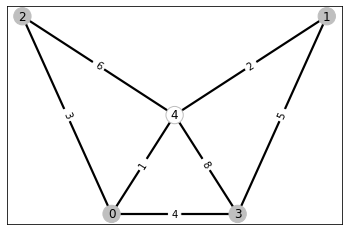
\includegraphics[width = 0.7\linewidth]{surface/matching.png}
    \caption{The resulting graph of the conversion of all X syndrome measurements to the matching problem. Each edge corresponds to a data qubit in the original circuit; each vertex corresponds to an ancilla of X syndrome measurement.}
    \label{fig:my_label}
\end{figure}

To briefly test the efficacy of the error-correcting surface code, we apply different error to the circuit and perform 1024 runs. Then compare the direct measurement result with the error correcting result. All circuits are initialized so that if we were to measure along the logical Z axis, it would always return $\ket{0}$. Some gates were then applied to simulated certain quantum circuit noise. A measurement at Z-logical axis is performed at the end, and the number of $\ket{0}$ and $\ket{1}$ measurements are recorded.

The error-correction step is then taken on the output depending on the initial and final ancilla bits measurements. The numbers of $\ket{0}$ and $\ket{1}$ after the correction are also recorded. Since in the case of a noise-free circuit, the measurement is always $\ket{0}$, the differences of the counts between the initial and error corrected measurement could serve an approximation of the efficacy of the surface code at error correction.

The result of surface code falls well within expectation. The code could correct any arbitrary Pauli error on a single qubit seemingly with 100\% accuracy, since all incorrect measurement results are corrected after the error correction step. What is notable is that the circuit seems to also be able to handle any rotation around X, Y, or Z axis of the Bloch's sphere on the 3 measurement qubits, which is technically greater than the code distance of our surface code. This is shown in Fig.10 and Fig.11.

\begin{figure}[p]
    \centering
    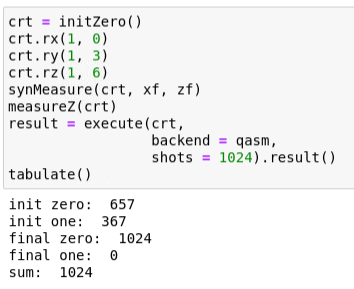
\includegraphics[width = 0.5\linewidth]{surface/rxryrz.PNG}
    \caption{The output of adding qubit rotation to 3 Z-logical qubits. The result shows all error being corrected.}
    \label{fig:my_label}
\end{figure}

\begin{figure}[p]
    \centering
    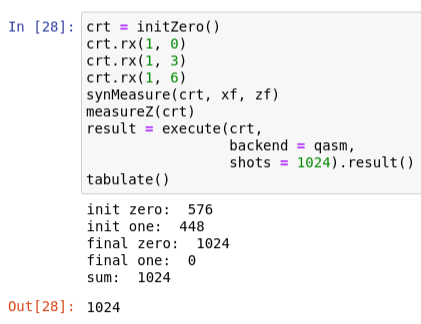
\includegraphics[width = 0.6\linewidth]{surface/rx-zl.PNG}
    \caption{The output of adding qubit rotation around x-axis to 3 Z-logical qubits. The result shows all error being corrected.}
    \label{fig:my_label}
\end{figure}

However, when applying rotation around the axes on the 3 X-logical qubits, the code merely reduces error, not correcting them. Examples are shown in Fig.12 and Fig.13. In this test, we apply 3 identical rotations around x-axis on the Bloch sphere on the 3 X-logical qubits, then measure the efficacy of the error-correction step against the input angle. The result is displayed in Fig.14. The circuit is initially not prone to error, then some minor errors are effectively corrected. However, the correction effectiveness quickly drops to 0 when the angle approaches $\pi/2$. What is interesting is that beyond $\theta = \pi/2$, the efficacy decreases to below 0, which means the surface code is generating more error than it corrects in the error-correcting step. However, the efficacy eventually level off to 0 as $\theta \xrightarrow{} \pi$.

\begin{figure}[h]
    \centering
    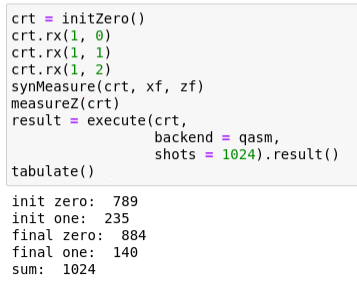
\includegraphics[width = 0.5\linewidth]{surface/rx-xl.PNG}
    \caption{The output of adding qubit rotation around x-axis to 3 X-logical qubits. The result shows errors being partially corrected.}
    \label{fig:my_label}
\end{figure}

\begin{figure}[h]
    \centering
    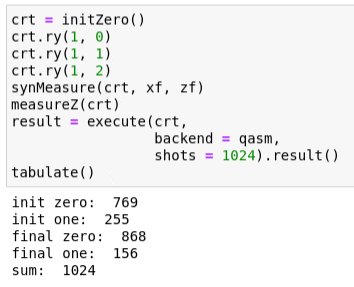
\includegraphics[width = 0.5\linewidth]{surface/ry-xl.PNG}
    \caption{The output of adding qubit rotation around y-axis to 3 X-logical qubits. The result shows errors being partially corrected.}
    \label{fig:my_label}
\end{figure}

\begin{figure}[h]
    \centering
    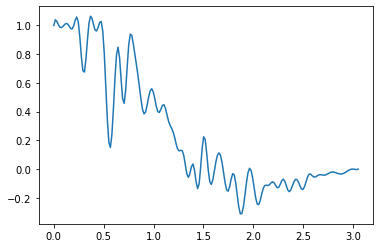
\includegraphics[width = 0.6\linewidth]{surface/efficacy_smoothed.png}
    \caption{Correction efficacy vs rotation angle. The x-axis denotes rotation angle in radian; the y-axis denotes error-correction efficacy. 1.0 denotes all errors corrected or no corrects needed, a number below 0 means the error-correction steps is correcting more errors than it fixes. The graph is smoothed with its nearest 2-neighbors.}
    \label{fig:my_label}
\end{figure}

\newpage
\section{Quantum Computing Simulator for Haskell}
In this section, we will briefly touch on the quantum computing simulator for Haskell. The code could be viewed at Ref.\cite{yanjunQaskell2021}

The simulator represents a circuit using its statevector, and any arbitrary gate / gates as a single transformation tensor on the entire circuit. The simulator serves several basic functions. These include: initializing a qubit to $\ket{0}$ state, or arbitrary state, initializing an array of qubit using a statevector, merging two set of qubits into one circuit, merging two transformation tensors into one, applying transformation tensor to circuit, applying a gate to a single qubit, applying controlled gate from a control qubit to an application qubit, and getting the probability of measuring $\ket{0}$ or $\ket{1}$ for any qubit of the circuit.

Since this version is coded and compiled under vanilla GHC, some extensive functions cannot be implemented as of right now. However, future development would implement functionalities including measure (collapsing state space), double control (Toffoli) gate, noise generation, custom gates, etc.

\section{Conclusion}

Through the numerous chapters in the paper, we discussed some interesting properties of the quantum gate, and briefly analyzed functions and properties of Qiskit when simulating quantum circuit on a traditional machine. Due to the lack of availability of physical quantum machines, the paper could provide some insight in navigating the landscape of quantum computing simulations on classical machines for beginners. In conclusion, this exploratory study could serve as an excellent foundation in our pursuit of better quantum algorithms.

\newpage
\appendix
\appendixpage
\section{Qiskit}

Qiskit is a python module for simulating quantum computation on classical machines. We will be using Qiskit in Jupyter Notebook for its convenience in organizing outputs an being able to run code in snippets. For this purpose the latest anaconda distribution was installed. Qiskit module could installed using the corresponding Python package manager, pip in my case.

After installation, Qiskit could be referenced in Jupyter Notebook using import command. Importing everything should be sufficient for simple circuit simulations. However, additional modules need to be imported if the user would like to send his circuit to be run on a physical quantum computer.

Creating a quantum circuit could be used using the function \newline$QuantumCircuit(,)$. The two arguments could be two integers greater than 0, or two list objects. The function returns a $QuantumCircuit$ object. Adding gates is linearly operated using $[QuantumCircuit].[gateName]()$, which takes one or more qubits, and there is no qiskit operation to delete the gate. However, since the $QuantumCircuit$ is a data object, we can use \newline$[QuantumCircuit].data.pop()$ operation to get rid of any gate of one's choosing. To see the circuit one has built, one could use $print()$ function. To see a beautified version, matplotlib could be used using the method \newline$[QuantumCircuit].draw(output='mpl')$.

Qiskit offers several different elements. These include Terra that is the circuit building component, Aer for simulation on conventional machines, Ignis for error correction, and Aqua to build realworld application. We will mainly use qasm (quantum assembly) simulator offered by Aer in our computations for its ease of use and not having to take up important computational resources. However, other simulators including statevector\_simulator and unitary\_simulator could also be obtained using Aer.get\_backend() function.

The circuit is run using the execute() function. The minimum requirement is the input circuit and the backend. The backend here could either be a simulator or a physical machine.

\newpage
\printbibliography

\end{document}